\begin{figure}
\centering
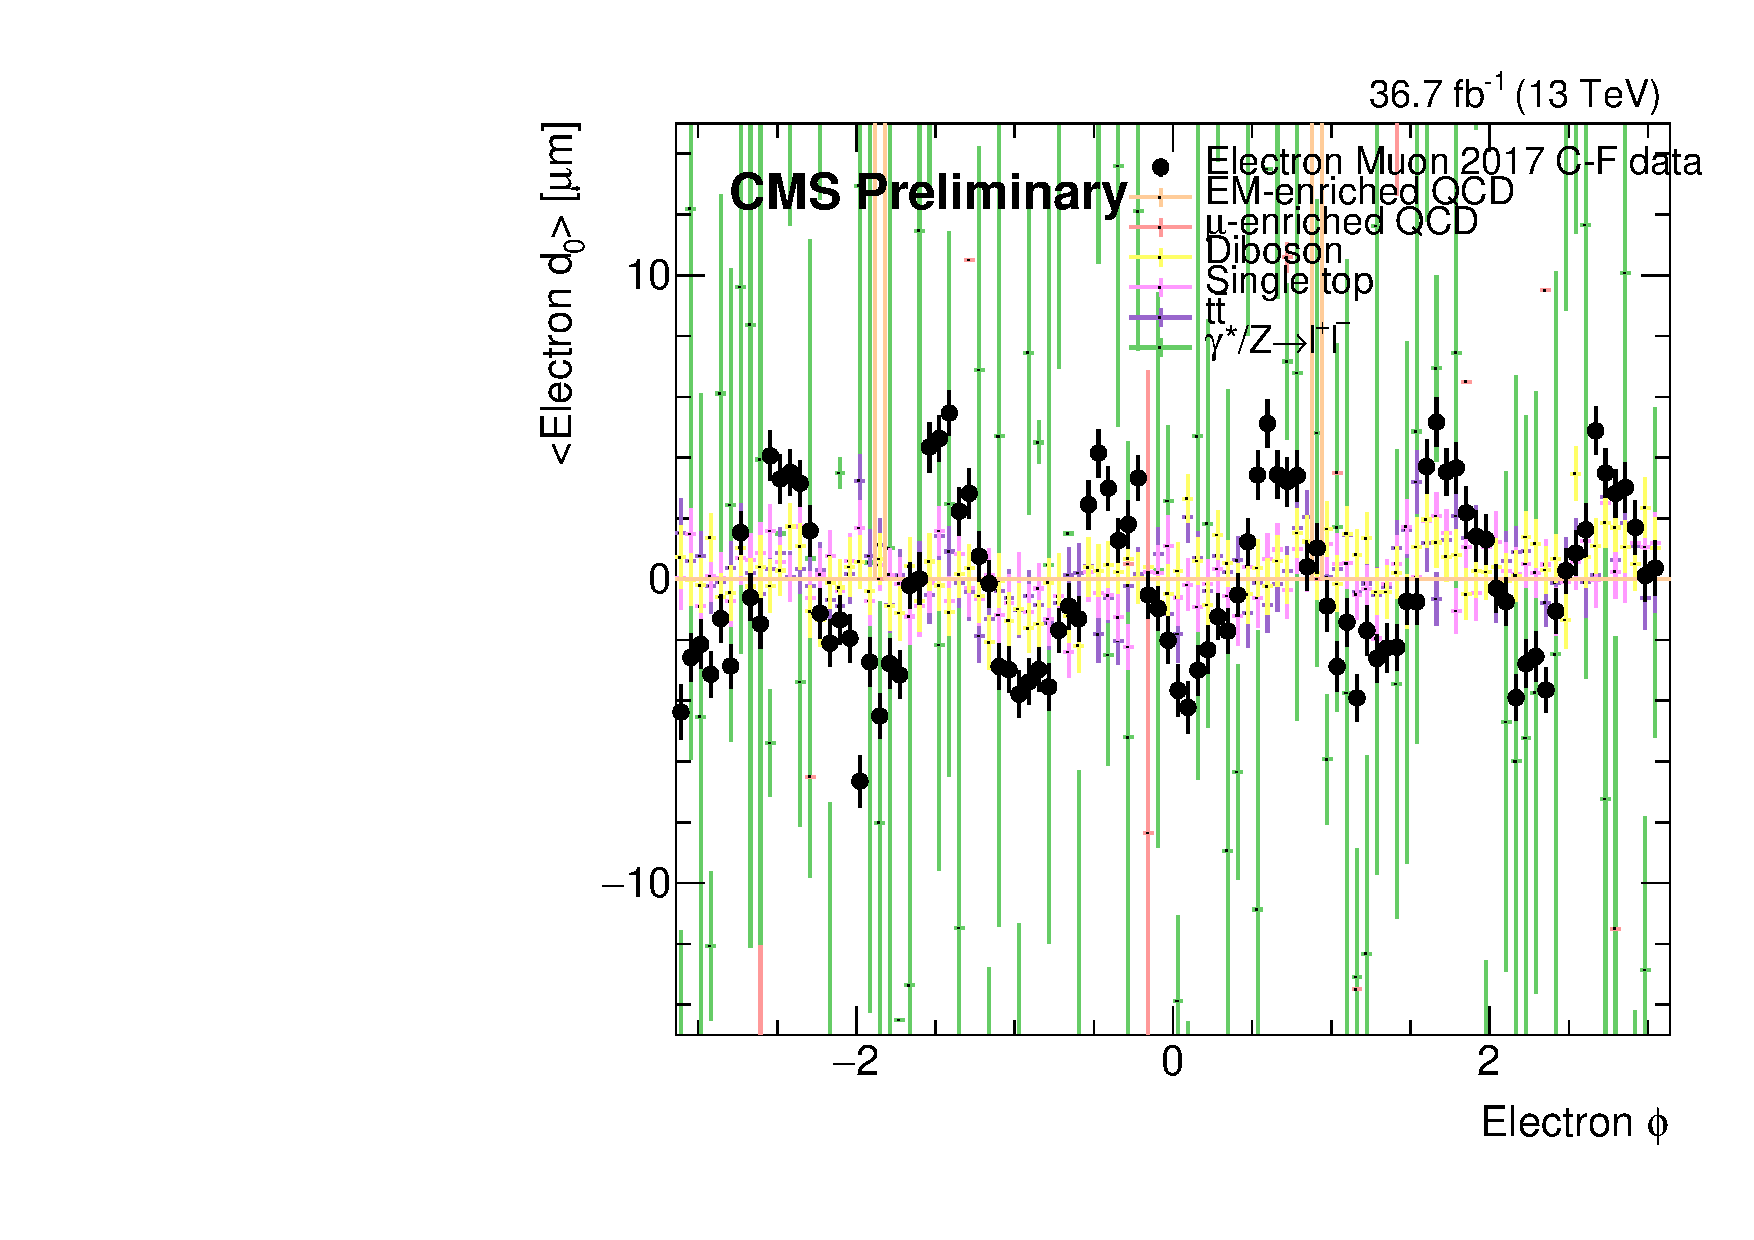
\includegraphics[width=0.4\textwidth]{figures/corrections/d0_smearing/emu_2017/electronD0_50um_vs_electronPhi_pfx.pdf}
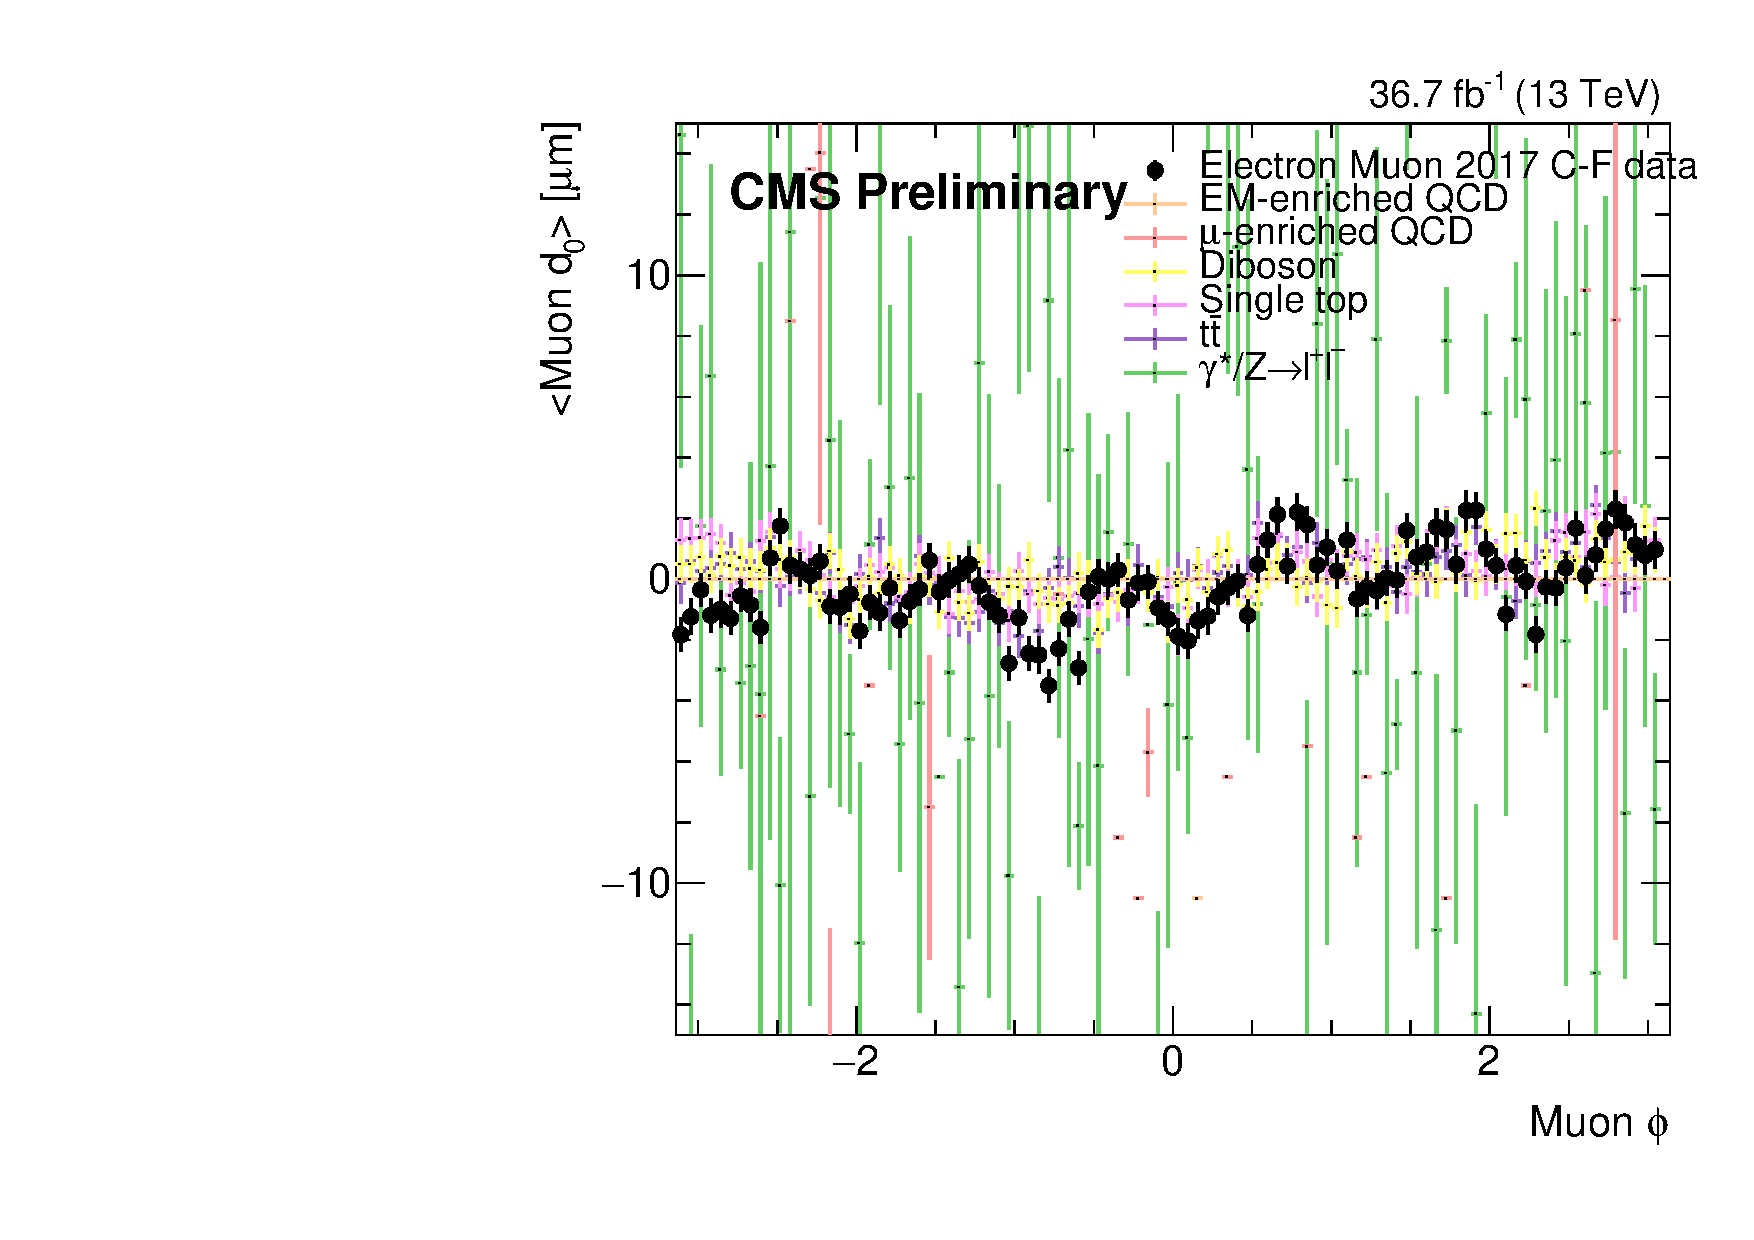
\includegraphics[width=0.4\textwidth]{figures/corrections/d0_smearing/emu_2017/muonD0_50um_vs_muonPhi_pfx.pdf}
\caption{The average lepton \ad as a function of $\phi$ in the $\Pe\Pgm$ prompt control region, for electrons (left) and muons (right), for 2017 data and simulation.}
\label{uncorrected_avg_d0_vs_phi}
\end{figure}

\begin{figure}
\centering
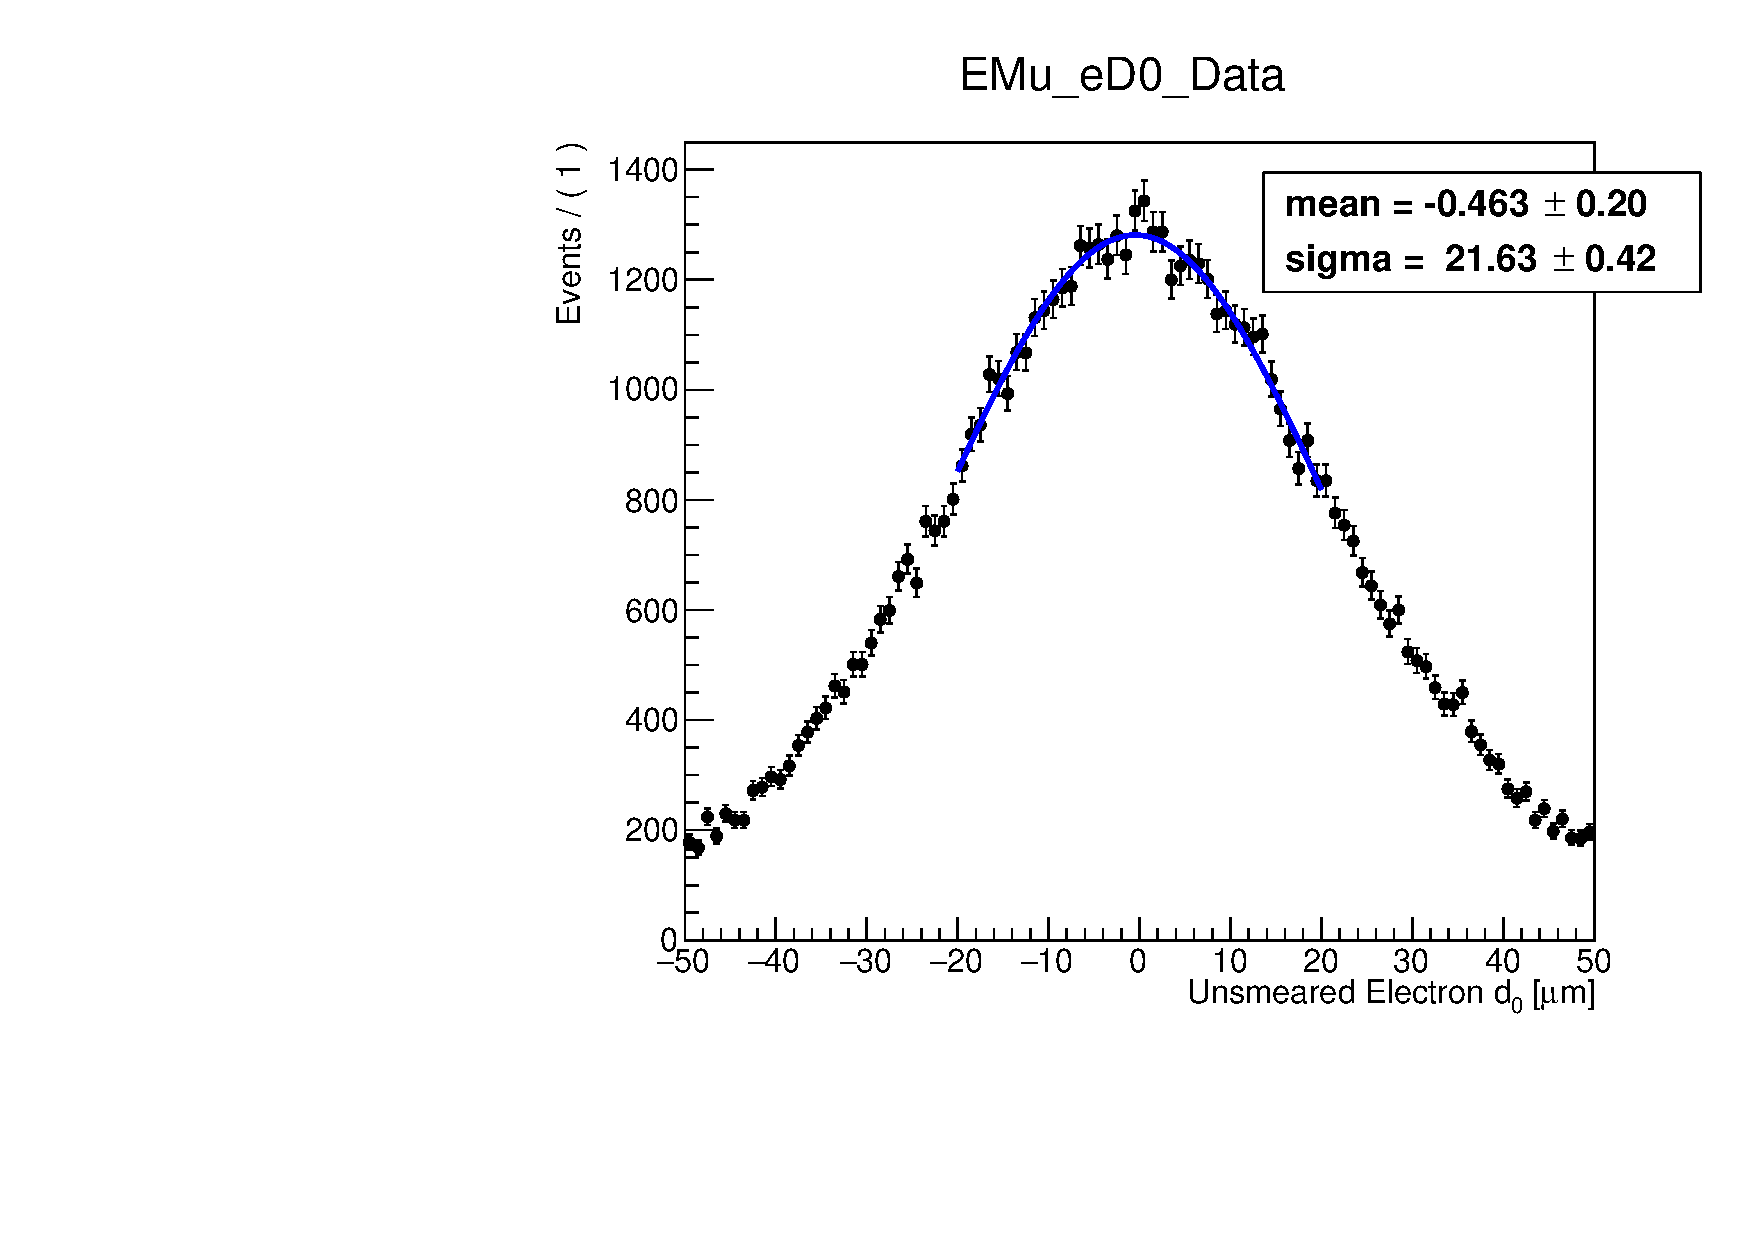
\includegraphics[width=0.24\textwidth]{figures/corrections/d0_smearing/emu_2017/gaussian_fit_EMu_eD0_Data.pdf}
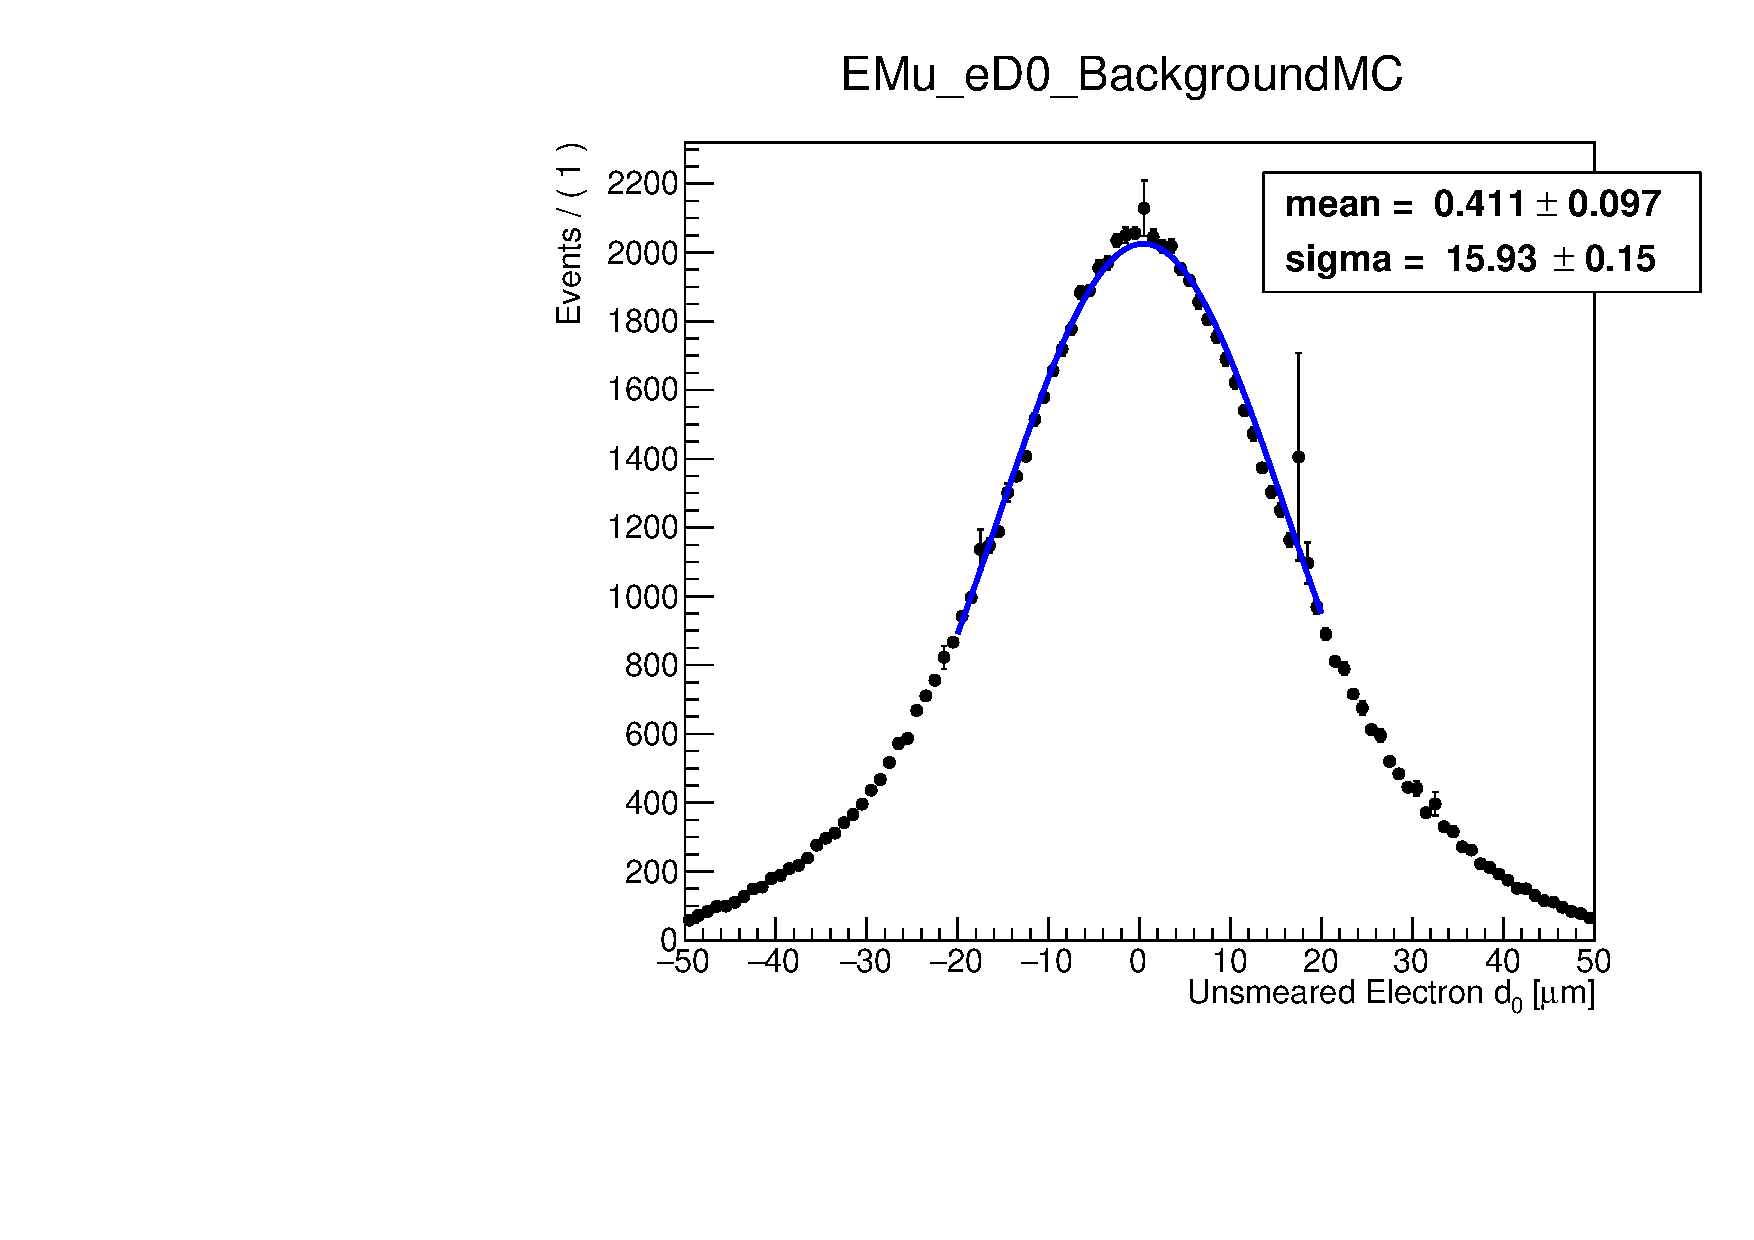
\includegraphics[width=0.24\textwidth]{figures/corrections/d0_smearing/emu_2017/gaussian_fit_EMu_eD0_BackgroundMC.pdf}
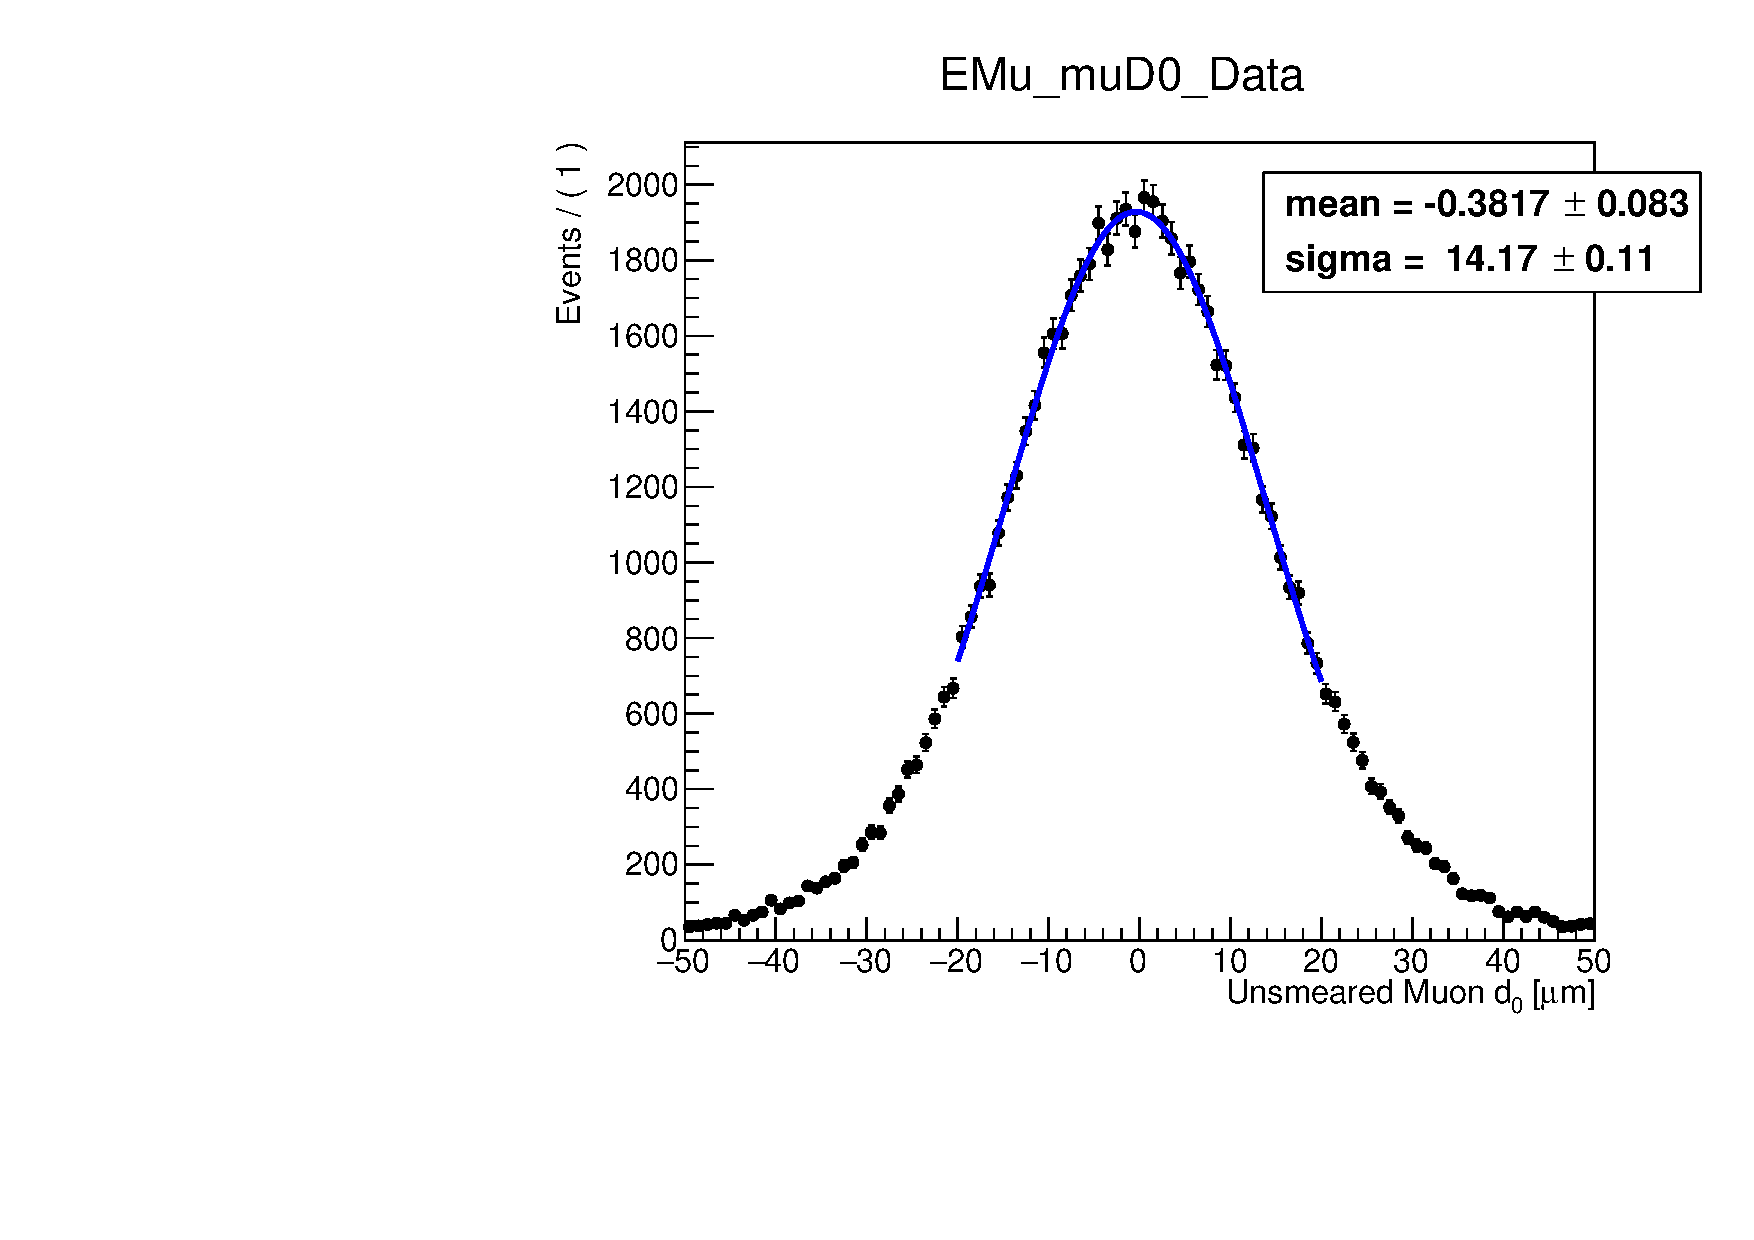
\includegraphics[width=0.24\textwidth]{figures/corrections/d0_smearing/emu_2017/gaussian_fit_EMu_muD0_Data.pdf} 
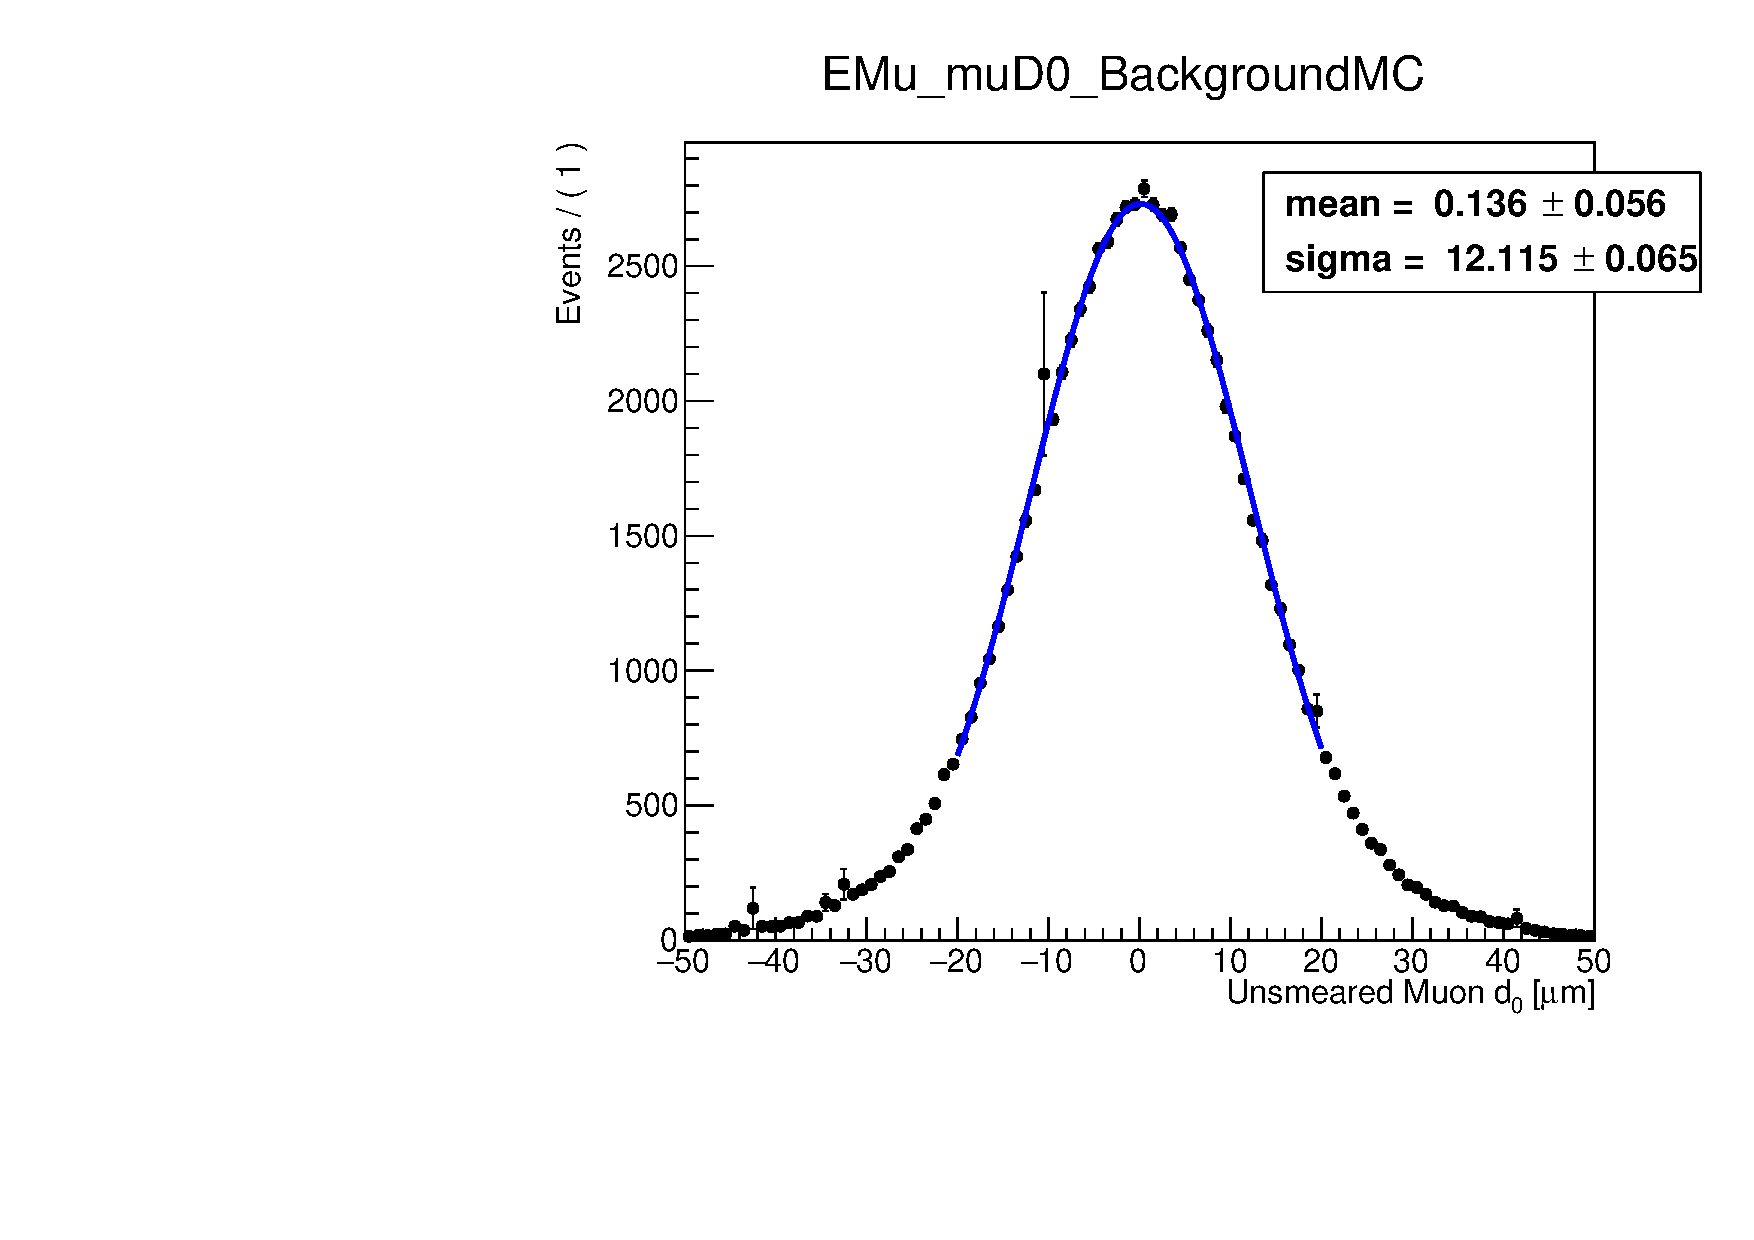
\includegraphics[width=0.24\textwidth]{figures/corrections/d0_smearing/emu_2017/gaussian_fit_EMu_muD0_BackgroundMC.pdf}
\caption{The lepton $d_0$ distributions with Gaussian fits in the 2017 $\Pe\Pgm$ prompt control region for (working from left to right) electrons in data, electrons in background simulation, muons in data, and muons in background simulation.}
\label{gaussian_fits_2017}
\end{figure}

\begin{figure}
\centering
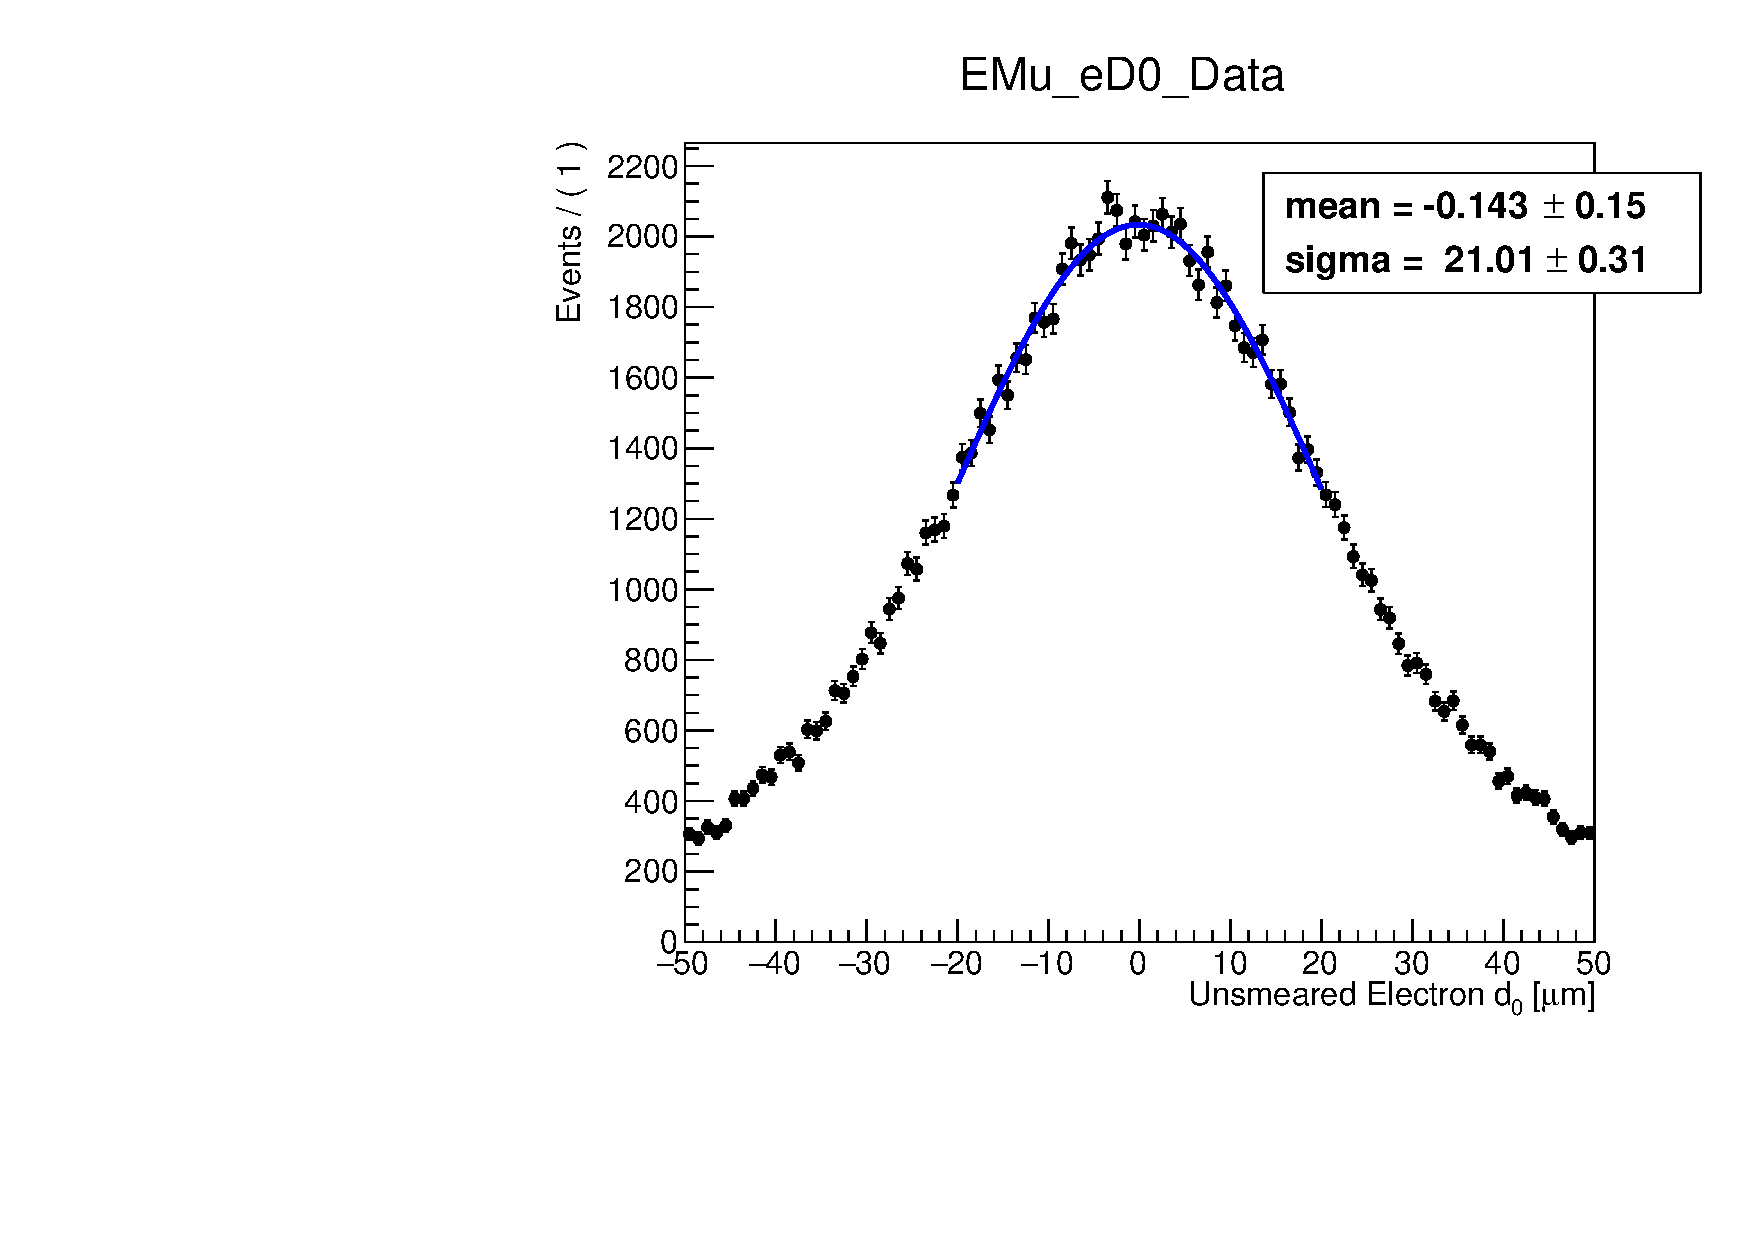
\includegraphics[width=0.24\textwidth]{figures/corrections/d0_smearing/emu_2018/gaussian_fit_EMu_eD0_Data.pdf}
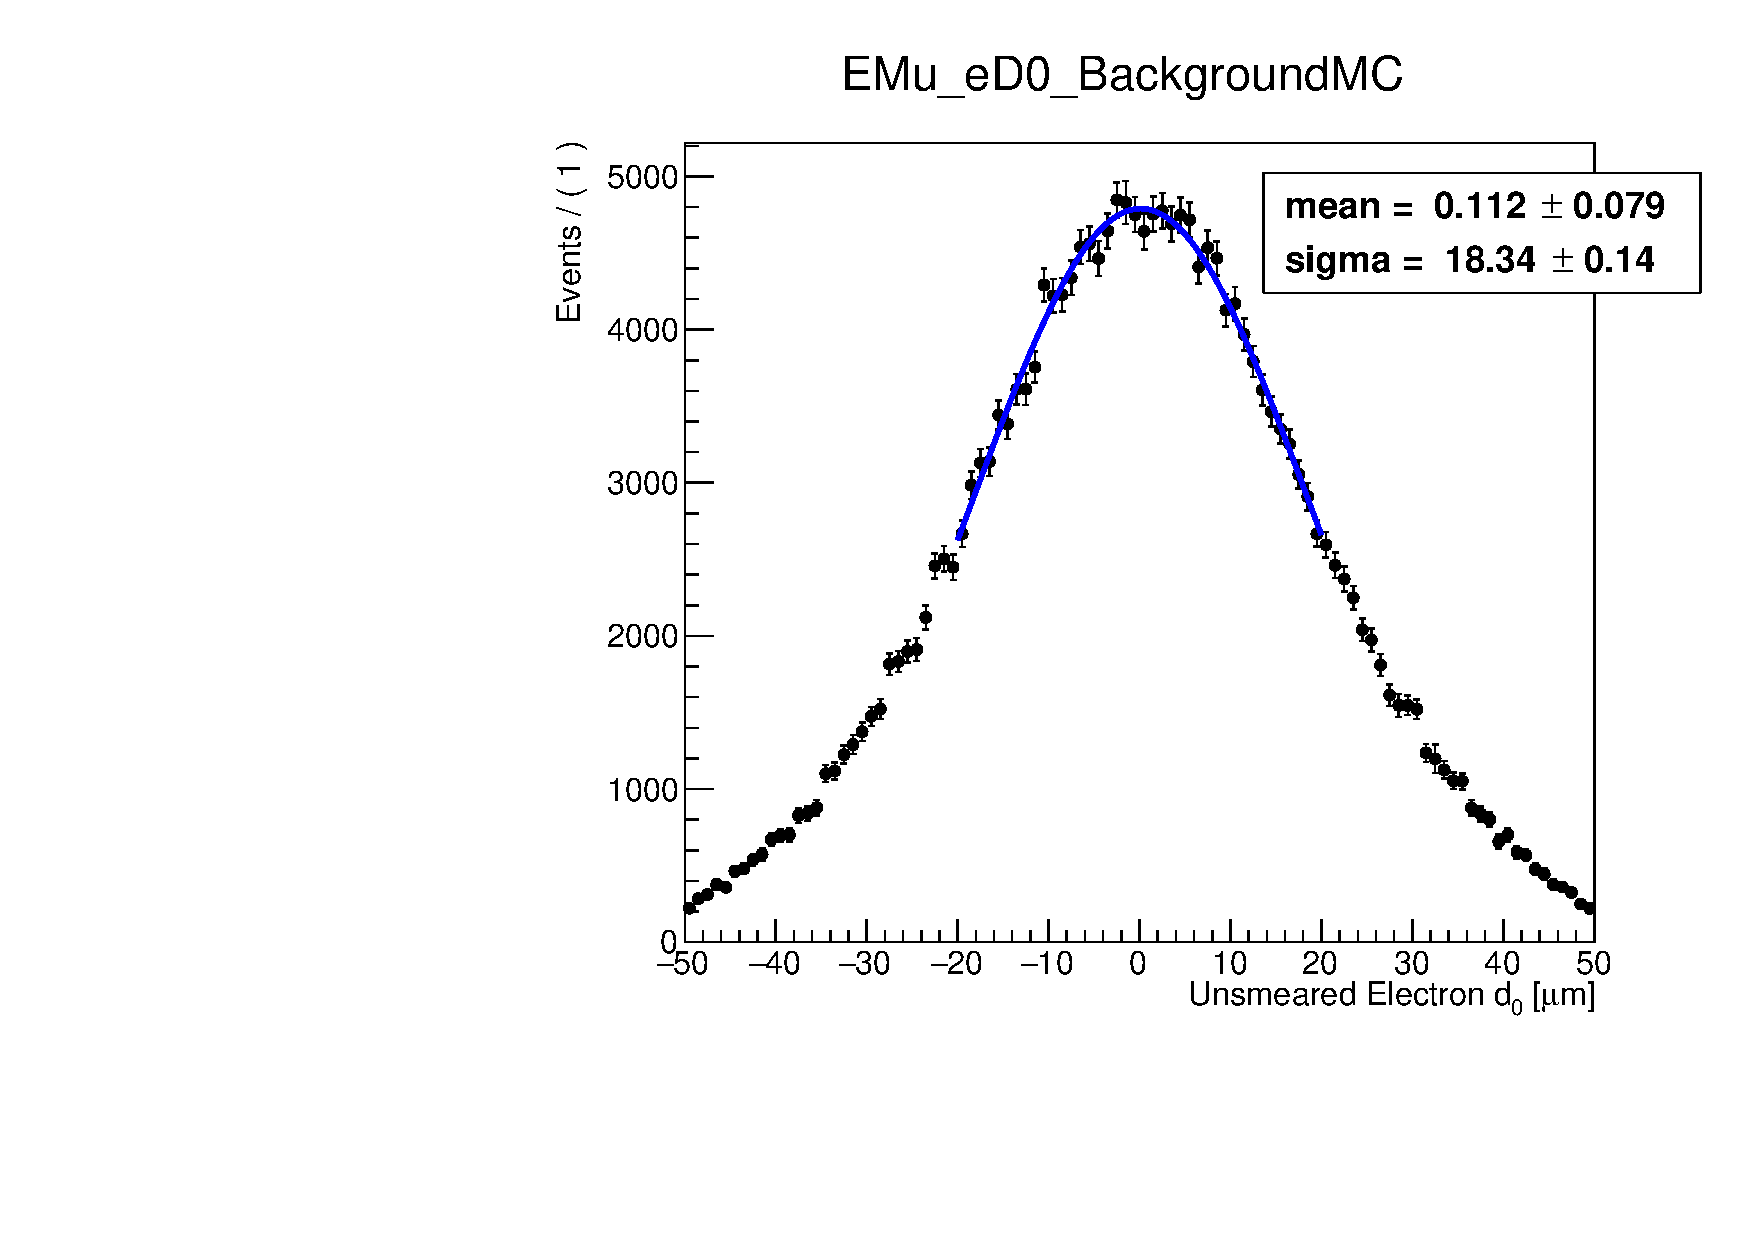
\includegraphics[width=0.24\textwidth]{figures/corrections/d0_smearing/emu_2018/gaussian_fit_EMu_eD0_BackgroundMC.pdf}
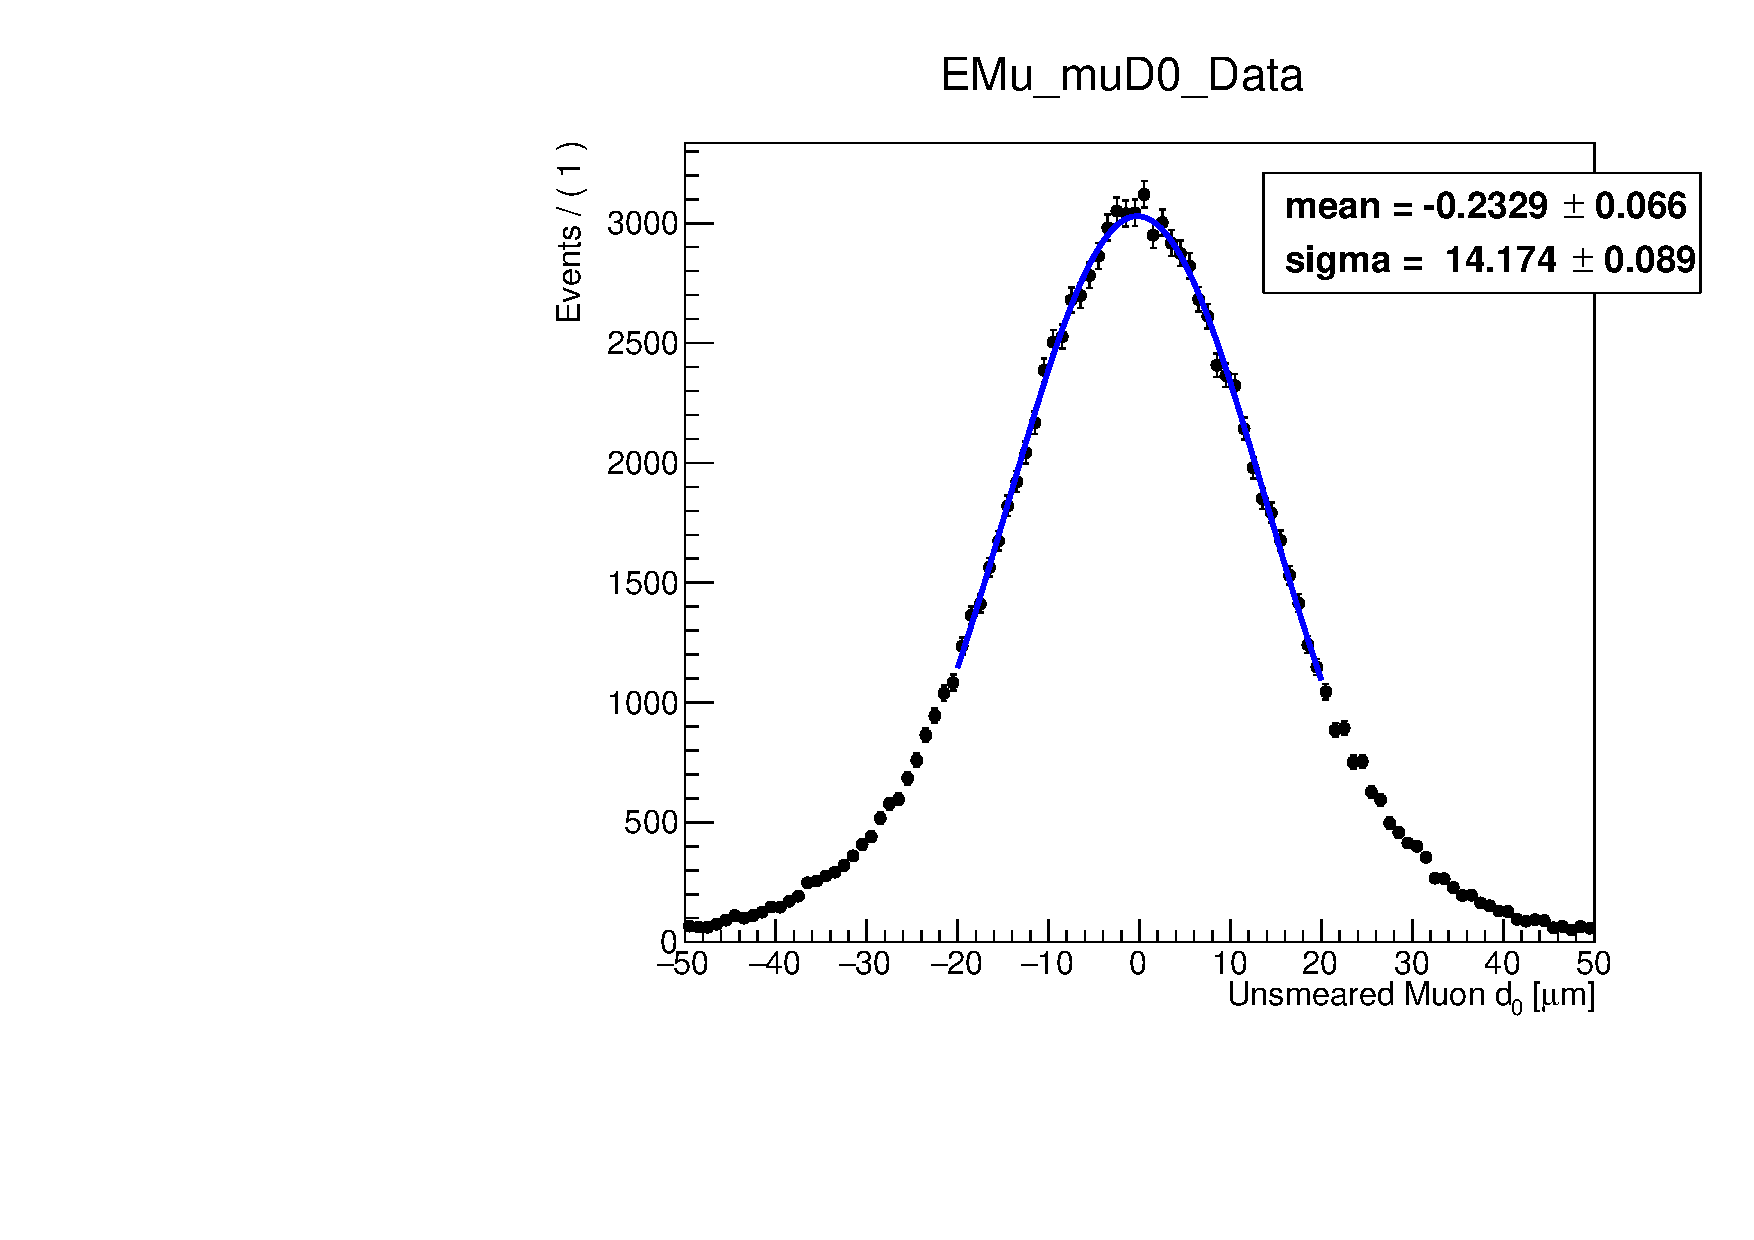
\includegraphics[width=0.24\textwidth]{figures/corrections/d0_smearing/emu_2018/gaussian_fit_EMu_muD0_Data.pdf} 
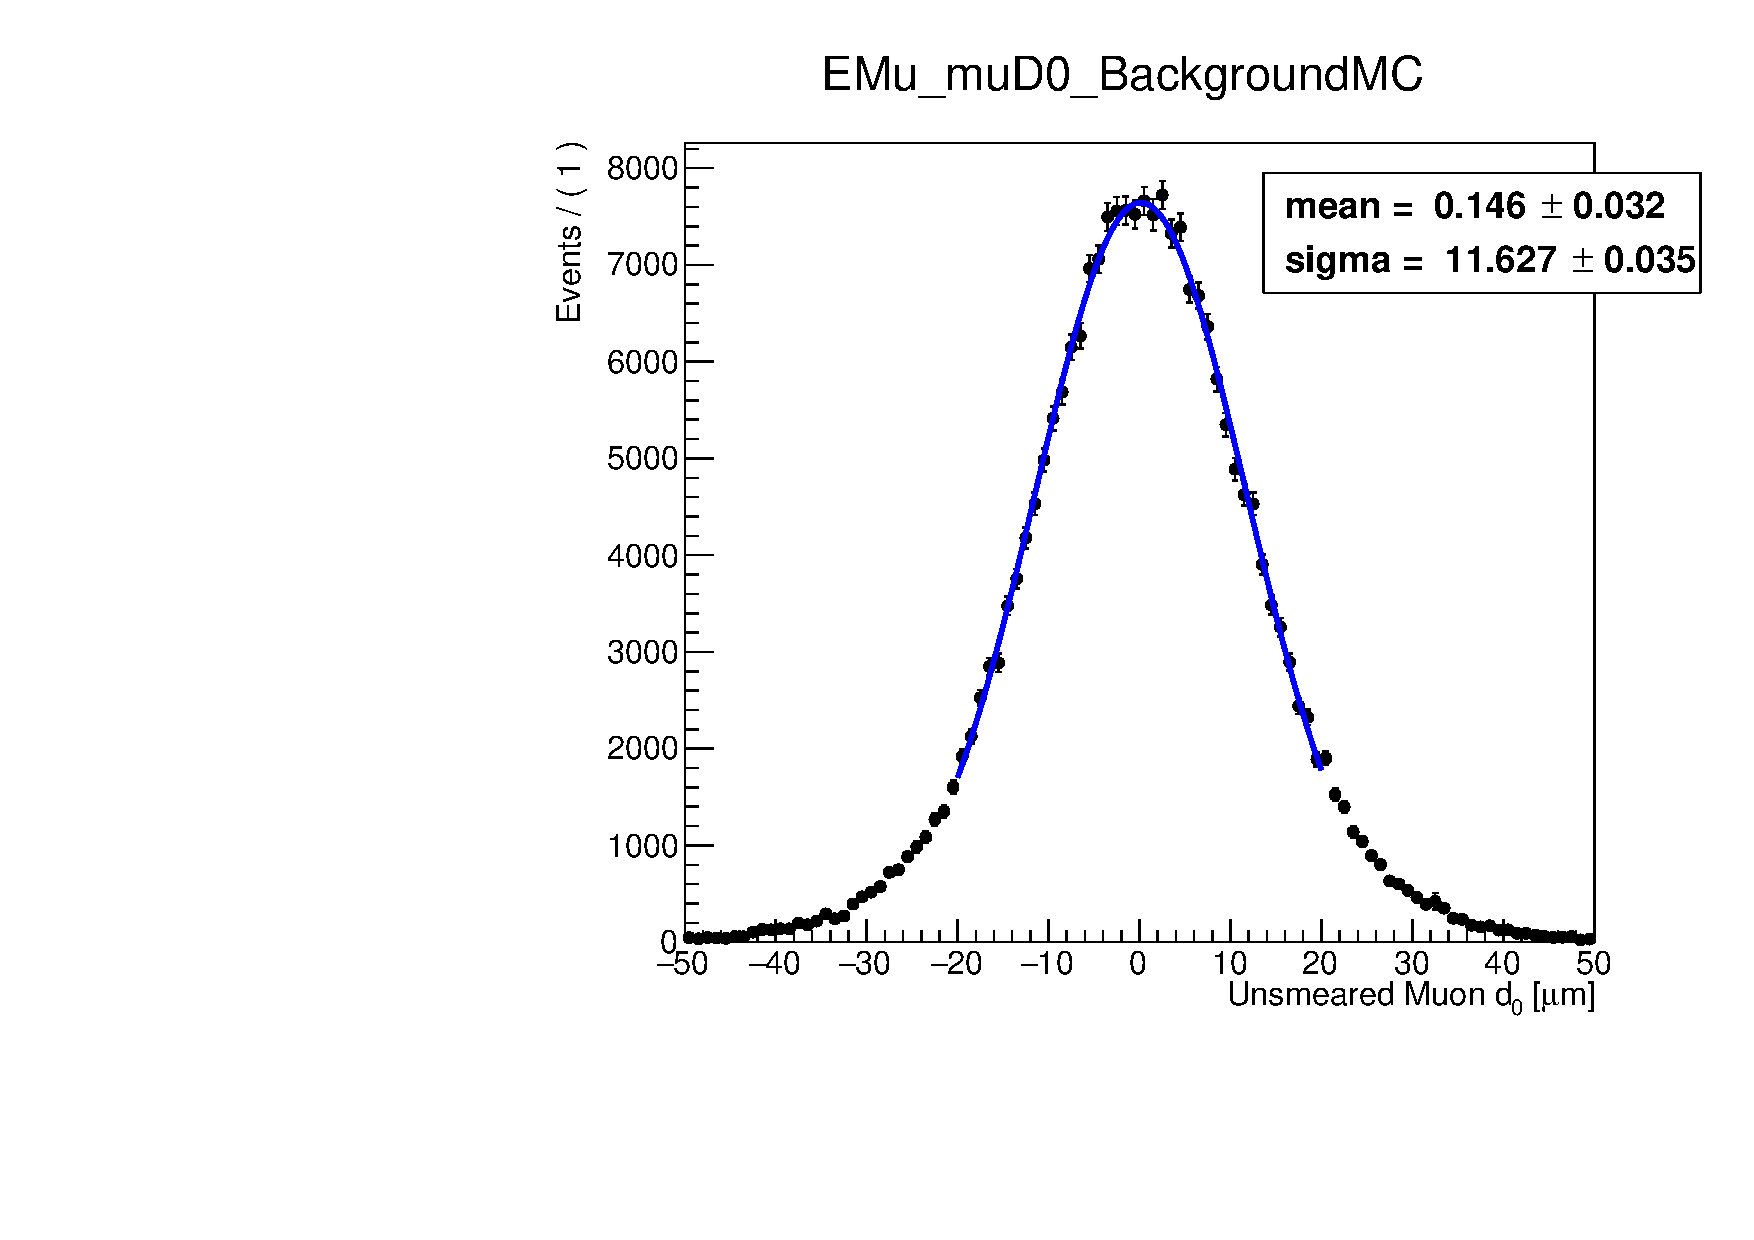
\includegraphics[width=0.24\textwidth]{figures/corrections/d0_smearing/emu_2018/gaussian_fit_EMu_muD0_BackgroundMC.pdf}
\caption{The lepton $d_0$ distributions with Gaussian fits in the 2018 $\Pe\Pgm$ prompt control region for (working from left to right) electrons in data, electrons in background simulation, muons in data, and muons in background simulation.}
\label{gaussian_fits_2018}
\end{figure}